\documentclass[a4paper,12pt]{article}

\usepackage[utf8]{inputenc}
\usepackage{amsmath}
\usepackage{graphicx}
\usepackage{float}
\usepackage{hyperref}

\title{Relatório sobre Conjuntos, Funções e Operadores Fuzzy}
\author{Doutorado CEFET}
\date{\today}

\begin{document}

\maketitle

\section{Introdução}
Este relatório apresenta a implementação e análise de funções de pertinência, fuzzificação, operações fuzzy e relações fuzzy. As funções de pertinência são amplamente utilizadas em lógica fuzzy para representar graus de pertencimento de elementos a conjuntos fuzzy.

\section{Funções de Pertinência}
\subsection{Implementação de Funcões de Pertinência}
As funções de pertinência implementadas incluem:

\subsubsection{Função Triangular}
A função triangular é definida por três parâmetros $(a, b, c)$, onde:
\begin{itemize}
    \item $a$ é o ponto inicial onde a pertinência começa a aumentar;
    \item $b$ é o ponto onde a pertinência atinge o valor máximo (1);
    \item $c$ é o ponto final onde a pertinência retorna a 0.
\end{itemize}
A fórmula é dada por:
\[
\mu(x) =
\begin{cases}
\frac{x - a}{b - a}, & \text{se } a \leq x < b, \\
\frac{c - x}{c - b}, & \text{se } b \leq x < c, \\
0, & \text{caso contrário.}
\end{cases}
\]
O código Python correspondente é:
\begin{verbatim}
def triangular(x, a, b, c):
    if a <= x < b:
        return (x - a) / (b - a)
    elif b <= x < c:
        return (c - x) / (c - b)
    else:
        return 0
\end{verbatim}
\begin{figure}[H]
    \centering
    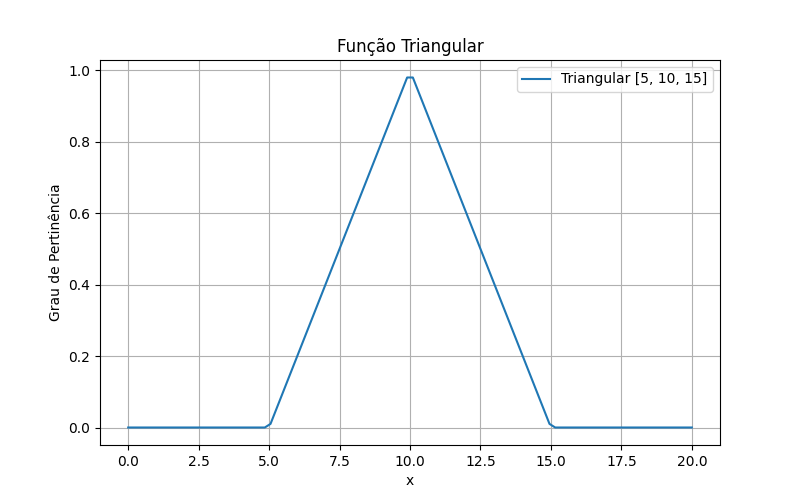
\includegraphics[width=0.8\textwidth]{img/triangular.png}
    \caption{Exemplo de função triangular com $a=5$, $b=10$, $c=15$.}
\end{figure}

\subsubsection{Função Trapezoidal}
A função trapezoidal é definida por quatro parâmetros $(a, b, c, d)$, onde:
\begin{itemize}
    \item $a$ e $d$ são os pontos onde a pertinência é 0;
    \item $b$ e $c$ definem a região onde a pertinência é 1.
\end{itemize}
A fórmula é:
\[
\mu(x) =
\begin{cases}
\frac{x - a}{b - a}, & \text{se } a \leq x < b, \\
1, & \text{se } b \leq x \leq c, \\
\frac{d - x}{d - c}, & \text{se } c < x \leq d, \\
0, & \text{caso contrário.}
\end{cases}
\]
O código Python correspondente é:
\begin{verbatim}
def trapezoidal(x, a, b, c, d):
    if a <= x < b:
        return (x - a) / (b - a)
    elif b <= x <= c:
        return 1
    elif c < x <= d:
        return (d - x) / (d - c)
    else:
        return 0
\end{verbatim}
\begin{figure}[H]
    \centering
    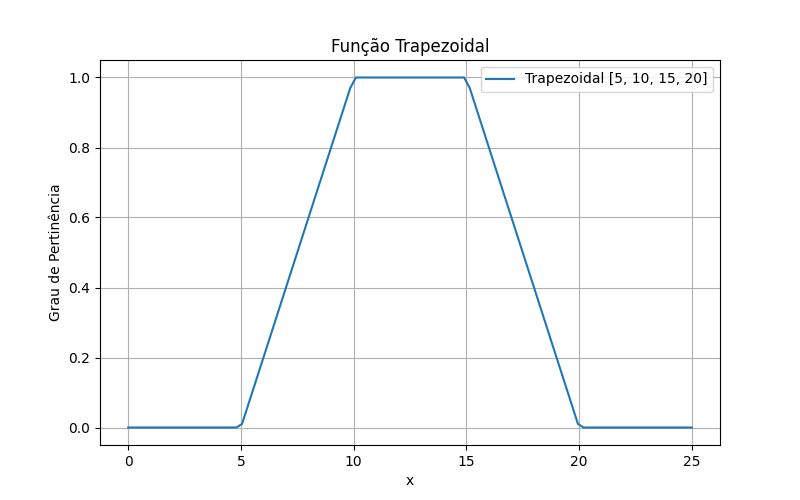
\includegraphics[width=0.8\textwidth]{img/trapezoidal.png}
    \caption{Exemplo de função trapezoidal com $a=5$, $b=10$, $c=15$, $d=20$.}
\end{figure}

\subsubsection{Função Gaussiana}
A função gaussiana é definida por dois parâmetros $(c, \sigma)$, onde:
\begin{itemize}
    \item $c$ é o centro da curva, onde a pertinência é máxima (1);
    \item $\sigma$ controla a largura da curva.
\end{itemize}
A fórmula é:
\[
\mu(x) = e^{-\frac{1}{2} \left( \frac{x - c}{\sigma} \right)^2}.
\]
O código Python correspondente é:
\begin{verbatim}
def gaussian(x, c, sigma):
    return np.exp(-0.5 * ((x - c) / sigma) ** 2)
\end{verbatim}
\begin{figure}[H]
    \centering
    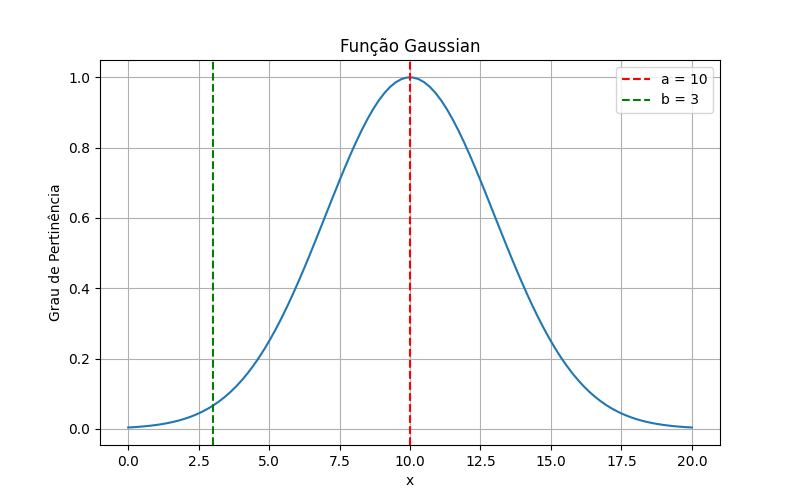
\includegraphics[width=0.8\textwidth]{img/gaussian.png}
    \caption{Exemplo de função gaussiana com $c=10$, $\sigma=3$.}
\end{figure}

\subsubsection{Função Sigmoidal}
A função sigmoidal é definida por dois parâmetros $(a, c)$, onde:
\begin{itemize}
    \item $a$ controla a inclinação da curva;
    \item $c$ é o ponto central onde a pertinência é 0.5.
\end{itemize}
A fórmula é:
\[
\mu(x) = \frac{1}{1 + e^{-a(x - c)}}.
\]
O código Python correspondente é:
\begin{verbatim}
def sigmoidal(x, a, c):
    return 1 / (1 + np.exp(-a * (x - c)))
\end{verbatim}
\begin{figure}[H]
    \centering
    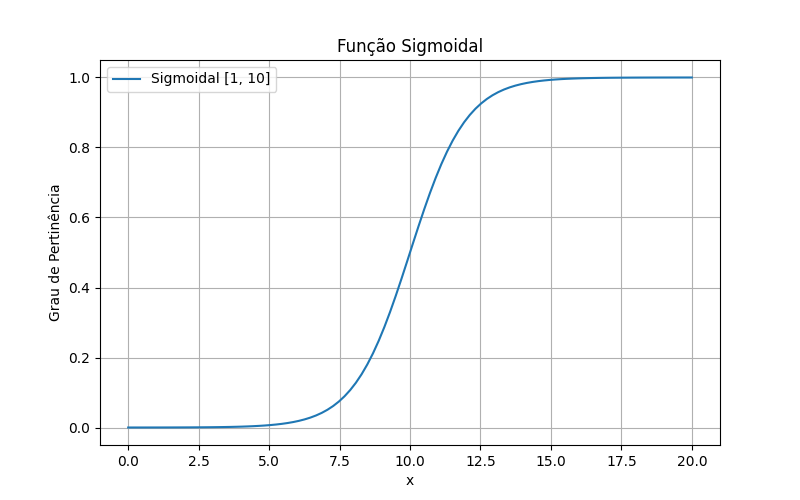
\includegraphics[width=0.8\textwidth]{img/sigmoidal.png}
    \caption{Exemplo de função sigmoidal com $a=1$, $c=10$.}
\end{figure}

\subsubsection{Função Sinoidal (Bell)}
A função Bell é definida por três parâmetros $(a, b, c)$, onde:
\begin{itemize}
    \item $a$ controla a largura da curva;
    \item $b$ controla a inclinação;
    \item $c$ é o centro da curva.
\end{itemize}
A fórmula é:
\[
\mu(x) = \frac{1}{1 + \left|\frac{x - c}{a}\right|^{2b}}.
\]
O código Python correspondente é:
\begin{verbatim}
def bell_function(x, a, b, c):
    return 1 / (1 + abs((x - c) / a) ** (2 * b))
\end{verbatim}
\begin{figure}[H]
    \centering
    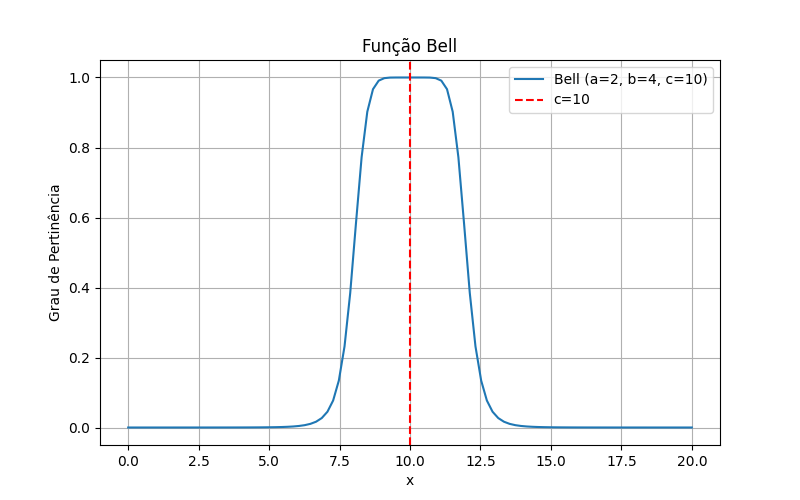
\includegraphics[width=0.8\textwidth]{img/bell.png}
    \caption{Exemplo de função Bell com $a=2$, $b=4$, $c=10$.}
\end{figure}

\subsubsection{Função S}
A função S é definida por dois parâmetros $(a, b)$, onde:
\begin{itemize}
    \item $a$ é o ponto onde a pertinência começa a aumentar;
    \item $b$ é o ponto onde a pertinência atinge 1.
\end{itemize}
A fórmula é:
\[
\mu(x) =
\begin{cases}
0, & \text{se } x \leq a, \\
2\left(\frac{x - a}{b - a}\right)^2, & \text{se } a < x < b, \\
1, & \text{se } x \geq b.
\end{cases}
\]
O código Python correspondente é:
\begin{verbatim}
def s_function(x, a, b):
    if x <= a:
        return 0
    elif a < x < b:
        return 2 * ((x - a) / (b - a)) ** 2
    elif x >= b:
        return 1
\end{verbatim}
\begin{figure}[H]
    \centering
    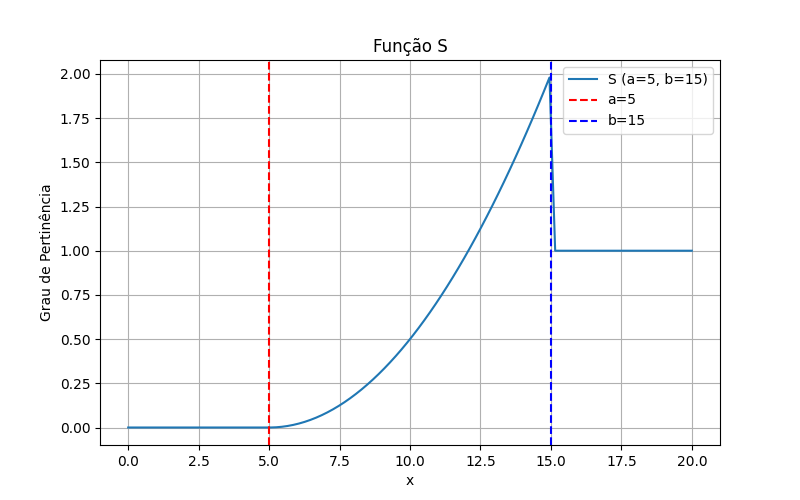
\includegraphics[width=0.8\textwidth]{img/s.png}
    \caption{Exemplo de função S com $a=5$, $b=15$.}
\end{figure}

\subsubsection{Função Z}
A função Z é definida por dois parâmetros $(a, b)$, onde:
\begin{itemize}
    \item $a$ é o ponto onde a pertinência começa a diminuir;
    \item $b$ é o ponto onde a pertinência atinge 0.
\end{itemize}
A fórmula é:
\[
\mu(x) =
\begin{cases}
1, & \text{se } x \leq a, \\
1 - 2\left(\frac{x - a}{b - a}\right)^2, & \text{se } a < x < b, \\
0, & \text{se } x \geq b.
\end{cases}
\]
O código Python correspondente é:
\begin{verbatim}
def z_function(x, a, b):
    if x <= a:
        return 1
    elif a < x < b:
        return 1 - 2 * ((x - a) / (b - a)) ** 2
    else:
        return 0
\end{verbatim}

\subsubsection{Função Cauchy}
A função Cauchy é definida por dois parâmetros $(c, \gamma)$, onde:
\begin{itemize}
    \item $c$ é o centro da curva;
    \item $\gamma$ controla a largura da curva.
\end{itemize}
A fórmula é:
\[
\mu(x) = \frac{1}{1 + \left(\frac{x - c}{\gamma}\right)^2}.
\]
O código Python correspondente é:
\begin{verbatim}
def cauchy_function(x, c, gamma):
    return 1 / (1 + ((x - c) / gamma) ** 2)
\end{verbatim}
\begin{figure}[H]
    \centering
    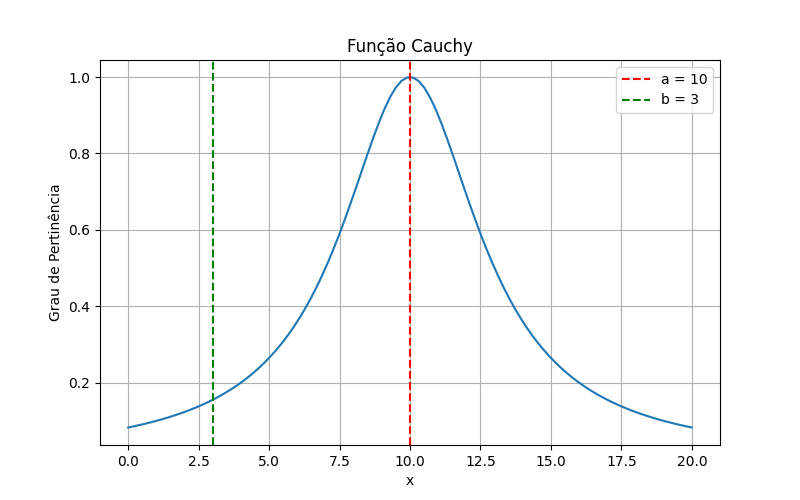
\includegraphics[width=0.8\textwidth]{img/cauchy.png}
    \caption{Exemplo de função Cauchy com $c=10$, $\gamma=3$.}
\end{figure}

\subsubsection{Função Gaussiana Dupla}
A função Gaussiana Dupla é definida por três parâmetros $(c, \sigma_1, \sigma_2)$, onde:
\begin{itemize}
    \item $c$ é o centro da curva;
    \item $\sigma_1$ controla a largura da curva para $x \leq c$;
    \item $\sigma_2$ controla a largura da curva para $x > c$.
\end{itemize}
A fórmula é:
\[
\mu(x) =
\begin{cases}
e^{-\frac{1}{2} \left( \frac{x - c}{\sigma_1} \right)^2}, & \text{se } x \leq c, \\
e^{-\frac{1}{2} \left( \frac{x - c}{\sigma_2} \right)^2}, & \text{se } x > c.
\end{cases}
\]
O código Python correspondente é:
\begin{verbatim}
def double_gaussian(x, c, sigma1, sigma2):
    if x <= c:
        return np.exp(-0.5 * ((x - c) / sigma1) ** 2)
    else:
        return np.exp(-0.5 * ((x - c) / sigma2) ** 2)
\end{verbatim}
\begin{figure}[H]
    \centering
    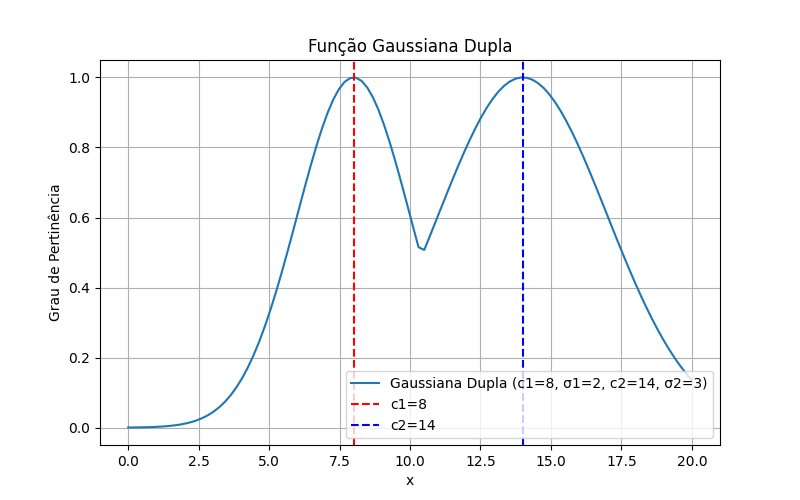
\includegraphics[width=0.8\textwidth]{img/double_gaussian.png}
    \caption{Exemplo de função Gaussiana Dupla com $c=10$, $\sigma_1=3$, $\sigma_2=5$.}
\end{figure}

\subsubsection{Função Logarítmica}
A função Logarítmica é definida por dois parâmetros $(a, b)$, onde:
\begin{itemize}
    \item $a$ controla o deslocamento da curva;
    \item $b$ controla a inclinação da curva.
\end{itemize}
A fórmula é:
\[
\mu(x) = 
\begin{cases}
0, & \text{se } x \leq a, \\
\log_b(x - a + 1), & \text{se } x > a.
\end{cases}
\]
O código Python correspondente é:
\begin{verbatim}
import math

def logarithmic_function(x, a, b):
    if x <= a:
        return 0
    else:
        return math.log(x - a + 1, b)
\end{verbatim}
\begin{figure}[H]
    \centering
    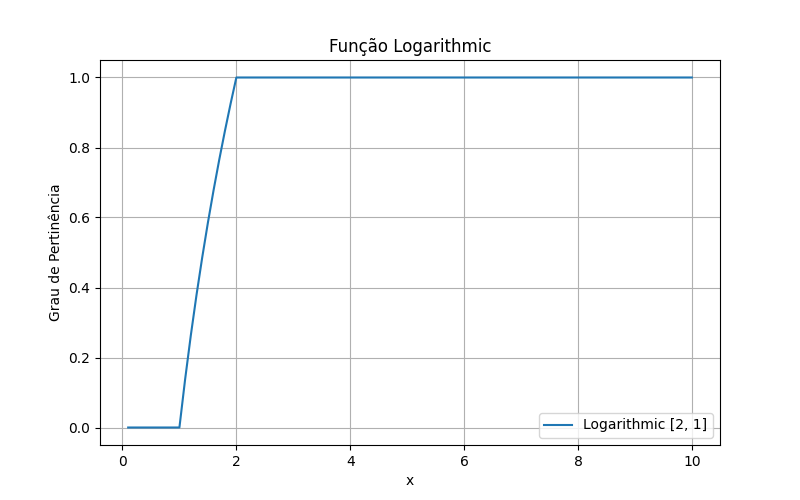
\includegraphics[width=0.8\textwidth]{img/logarithmic.png}
    \caption{Exemplo de função Logarítmica com $a=5$, $b=2$.}
\end{figure}

\subsubsection{Função Retangular}
A função Retangular é definida por dois parâmetros $(a, b)$, onde:
\begin{itemize}
    \item $a$ é o início do intervalo onde a pertinência é 1;
    \item $b$ é o final do intervalo onde a pertinência é 1.
\end{itemize}
A fórmula é:
\[
\mu(x) =
\begin{cases}
1, & \text{se } a \leq x \leq b, \\
0, & \text{caso contrário.}
\end{cases}
\]
O código Python correspondente é:
\begin{verbatim}
def rectangular(x, a, b):
    if a <= x <= b:
        return 1
    else:
        return 0
\end{verbatim}
\begin{figure}[H]
    \centering
    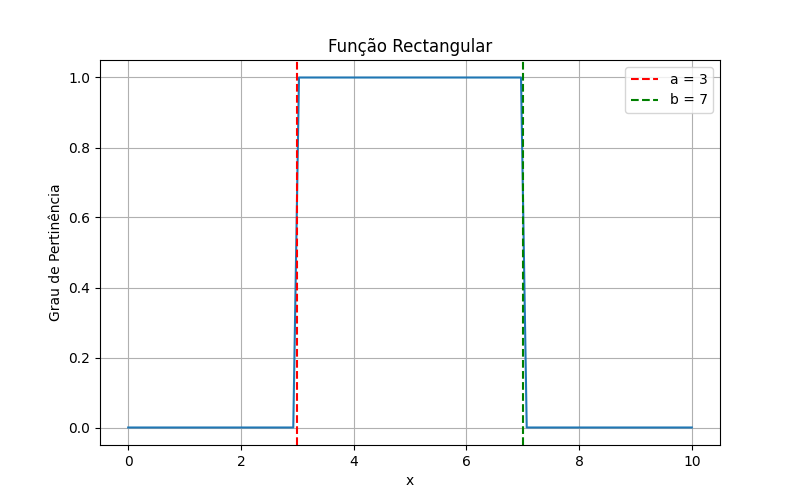
\includegraphics[width=0.8\textwidth]{img/rectangular.png}
    \caption{Exemplo de função Retangular com $a=10$, $b=20$.}
\end{figure}

\subsection{Fuzzificação e Análise Comparativa}
Para a fuzzificação, escolhemos uma variável de entrada com universo de discurso definido e particionamos o domínio em funções de pertinência uniformemente espaçadas. A seguir, apresentamos os resultados para duas amostras distintas.

Este relatório apresenta a definição de funções de pertinência fuzzy, a fuzzificação de amostras e a análise gráfica e textual dos resultados. As funções de pertinência analisadas incluem as funções triangular, trapezoidal, gaussiana e sigmoidal.

\section{Definição do Universo de Discurso}
A variável de entrada escolhida é a \textbf{temperatura ambiente}, com o universo de discurso definido como $[0, 40]$ graus Celsius.

\section{Particionamento do Domínio}
O domínio foi particionado em quatro funções de pertinência uniformemente espaçadas para cada tipo de função. Os parâmetros utilizados são descritos abaixo:

\subsection{Função Triangular}
\[
\mu_{\text{triangular}}(x; a, b, c) =
\begin{cases}
0, & x \leq a \text{ ou } x \geq c, \\
\frac{x - a}{b - a}, & a < x \leq b, \\
\frac{c - x}{c - b}, & b < x < c.
\end{cases}
\]
Parâmetros: $a = 0$, $b = 10$, $c = 20$; $a = 10$, $b = 20$, $c = 30$; $a = 20$, $b = 30$, $c = 40$.

\subsection{Função Trapezoidal}
\[
\mu_{\text{trapezoidal}}(x; a, b, c, d) =
\begin{cases}
0, & x \leq a \text{ ou } x \geq d, \\
\frac{x - a}{b - a}, & a < x \leq b, \\
1, & b < x \leq c, \\
\frac{d - x}{d - c}, & c < x < d.
\end{cases}
\]
Parâmetros: $a = 0$, $b = 5$, $c = 15$, $d = 20$; $a = 10$, $b = 15$, $c = 25$, $d = 30$; $a = 20$, $b = 25$, $c = 35$, $d = 40$.

\subsection{Função Gaussiana}
\[
\mu_{\text{gaussiana}}(x; c, \sigma) = \exp\left(-\frac{(x - c)^2}{2\sigma^2}\right)
\]
Parâmetros: $c = 10$, $\sigma = 5$; $c = 20$, $\sigma = 5$; $c = 30$, $\sigma = 5$.

\subsection{Função Sigmoidal}
\[
\mu_{\text{sigmoidal}}(x; a, c) = \frac{1}{1 + e^{-a(x - c)}}
\]
Parâmetros: $a = 1$, $c = 10$; $a = 1$, $c = 20$; $a = 1$, $c = 30$.

\section{Fuzzificação de Amostras}
As amostras escolhidas para fuzzificação foram $x = 15$ e $x = 25$. Os graus de ativação para cada função de pertinência foram calculados e apresentados nos gráficos a seguir.

\section{Resultados Gráficos}
Os gráficos abaixo mostram o universo de discurso, as funções de pertinência e os graus de ativação das amostras.

\subsection{Função Triangular}
\begin{figure}[H]
    \centering
    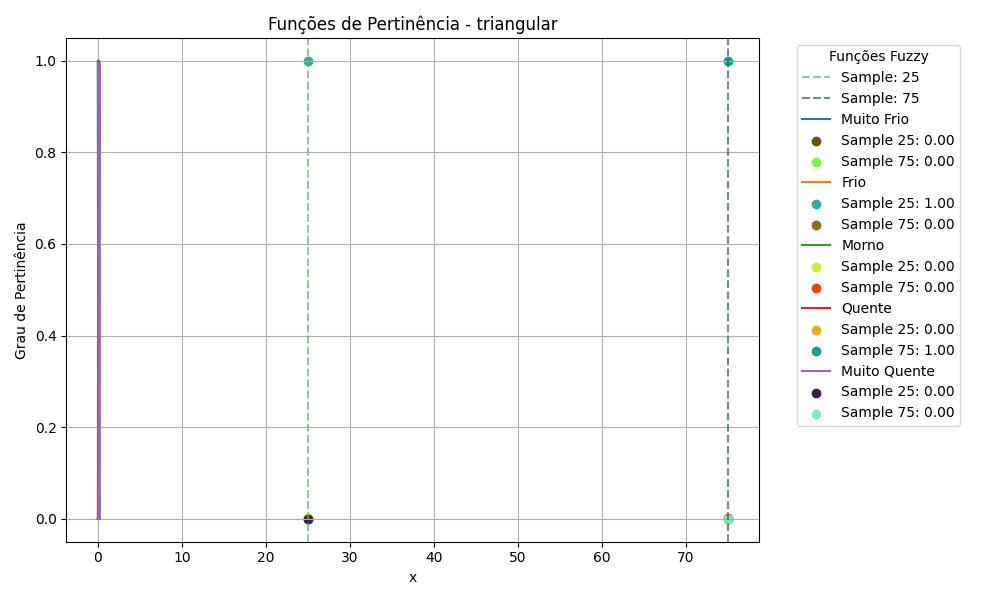
\includegraphics[width=0.8\textwidth]{img/funções_de_pertinência_triangular_fuzzificado.png}
    \caption{Funções de pertinência triangulares e graus de ativação.}
\end{figure}

\subsection{Função Trapezoidal}
\begin{figure}[H]
    \centering
    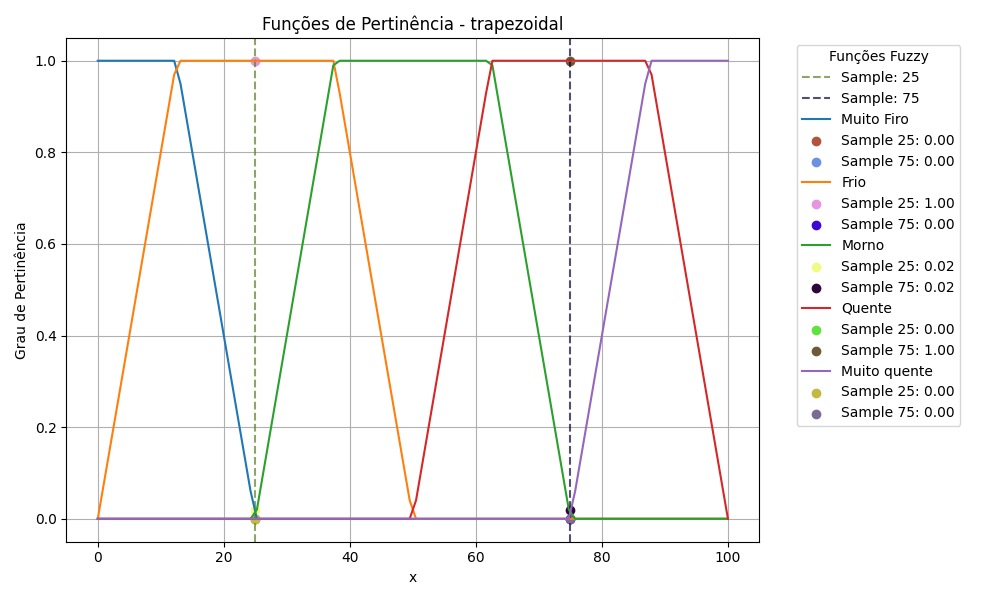
\includegraphics[width=0.8\textwidth]{img/funções_de_pertinência_trapezoidal_fuzzificado.png}
    \caption{Funções de pertinência trapezoidais e graus de ativação.}
\end{figure}

\subsection{Função Gaussiana}
\begin{figure}[H]
    \centering
    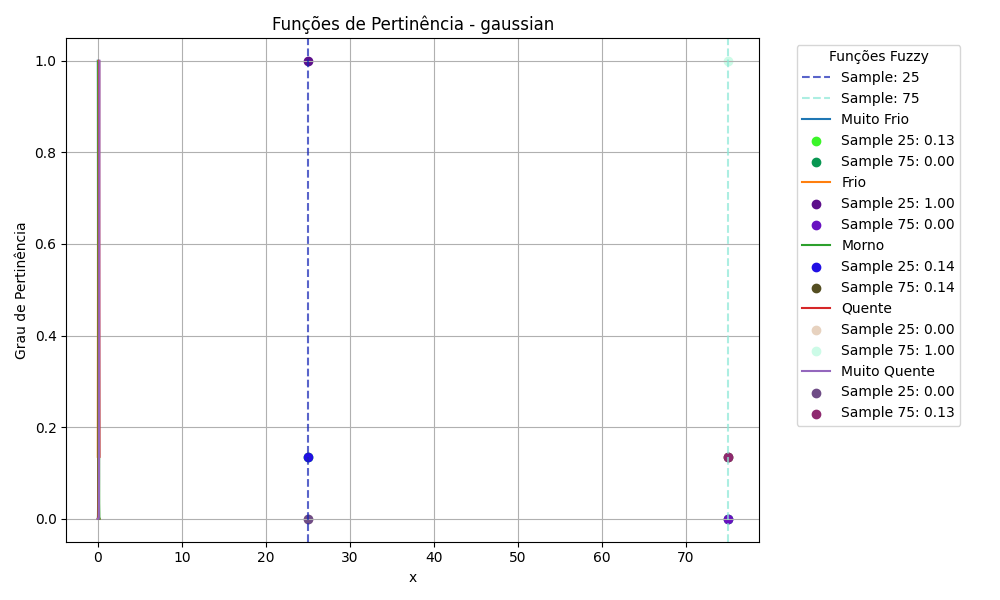
\includegraphics[width=0.8\textwidth]{img/funções_de_pertinência_gaussian_fuzzificado.png}
    \caption{Funções de pertinência gaussianas e graus de ativação.}
\end{figure}

\subsection{Função Sigmoidal}
\begin{figure}[H]
    \centering
    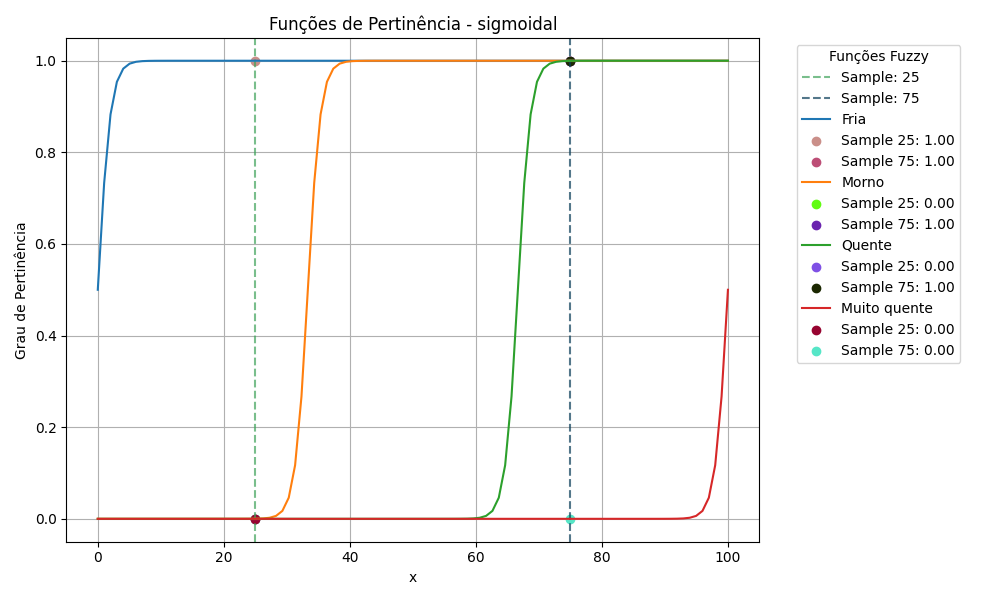
\includegraphics[width=0.8\textwidth]{img/funções_de_pertinência_sigmoidal_fuzzificado.png}
    \caption{Funções de pertinência sigmoidais e graus de ativação.}
\end{figure}

\section{Análise Comparativa}
\begin{itemize}
    \item As funções triangulares e trapezoidais apresentam transições mais abruptas entre os graus de pertinência, enquanto as funções gaussianas e sigmoidais possuem transições mais suaves.
    \item As funções gaussianas são mais sensíveis a variações próximas ao centro, enquanto as funções sigmoidais apresentam maior suavidade em todo o domínio.
    \item As funções trapezoidais são úteis para representar intervalos com pertinência máxima constante, enquanto as funções triangulares são mais adequadas para transições lineares.
\end{itemize}

\section{Conclusão}
Este relatório apresentou a definição, particionamento e análise de funções de pertinência para a variável temperatura ambiente. A análise gráfica e textual destacou as diferenças entre os tipos de funções, evidenciando suas características e aplicações.



\end{document}